\documentclass[12pt,a4paper]{report}

\usepackage{array}
\usepackage{makecell}
\usepackage{microtype}
\newcolumntype{L}[1]{>{\raggedright\let\newline\\\arraybackslash\hspace{0pt}}m{#1}}
\newcolumntype{C}[1]{>{\centering\let\newline\\\arraybackslash\hspace{0pt}}m{#1}}
\newcolumntype{R}[1]{>{\raggedleft\let\newline\\\arraybackslash\hspace{0pt}}m{#1}}

\usepackage{mathptmx}
\usepackage{graphicx} % Required for inserting images
\graphicspath{{img/}}
\usepackage{multirow}
\usepackage{caption}
\usepackage{longtable}


\usepackage{geometry}
\geometry{
	top=4cm,
	right=3cm,
	left=4cm,
	bottom=3cm,	
}

\usepackage{pdflscape}
\usepackage{tabularray}
\usepackage[table]{xcolor}
\usepackage{setspace}
\onehalfspacing
  
\renewcommand{\thechapter}{\centering \Roman{chapter}}
\renewcommand{\thesection}{\arabic{chapter}.\arabic{section}}

\def\contentsname{DAFTAR ISI}
\renewcommand\bibname{DAFTAR PUSTAKA}
\def\chaptername{BAB}

\usepackage{titlesec}
\titleformat{\chapter}[display]{\normalfont\bfseries\centering}{\MakeUppercase{\chaptertitlename}~\thechapter}{0pt}{}
\titlespacing*{\chapter}{0pt}{-2pt}{16pt}

\renewcommand{\arraystretch}{1.5}

\renewcommand\thechapter{\Roman{chapter}}
\renewcommand\thesection{\arabic{section}}
\def\thesection{\arabic{chapter}.\arabic{section}}
\def\thetable{\arabic{table}}

\titleformat{\section}[block]{\bf\normalsize}{\thesection}{0.6em}{}
\titlespacing*{\section}{0pt}{5pt}{0pt}
\titleformat{\subsection}[block]{\bf\normalsize}{\thesubsection}{0.6em}{}
\titlespacing*{\subsection}{0pt}{5pt}{0pt}

\usepackage{setspace}
%\singlespacing
\onehalfspacing
%\doublespacing
%\setstretch{1.1}
\renewcommand{\tablename}{Tabel}
\renewcommand{\figurename}{Gambar}
\renewcommand{\thefigure}{\thesection.\arabic{figure}}
\renewcommand{\thetable}{\thesection.\arabic{table}}
\usepackage[breaklinks]{hyperref}
\renewcommand{\listfigurename}{DAFTAR GAMBAR}
\renewcommand{\listtablename}{DAFTAR TABEL}

\hyphenation{me-la-in-kan}

\newcommand{\nim}{1990343054}							% NIM Mahasiswa 
\newcommand{\mahasiswa}{JUWANDA AZI MAYUSWA}	% Nama Mahasiswa
\newcommand{\judulId}{PENERAPAN FACE RECOGNITION DAN CLOUD COMPUTING PADA APLIKASI PRESENSI SMK NEGERI 1 KARANG BARU}
\newcommand{\judulEn}{Thesis Title}
\newcommand{\jurusan}{Jurusan Teknologi Informasi dan Komputer}
\newcommand{\prodi}{Teknologi Rekayasa Komputer Jaringan}
\newcommand{\institusi}{Politeknik Negeri Lhokseumawe}
\newcommand{\pembimbingUtama}{Indrawati, SST., M.T}
\newcommand{\nipPembimbingUtama}{197408152001122001}
\newcommand{\pembimbingPendamping}{Mahlil, S. Pd., M.A}
\newcommand{\nipPembimbingPendamping}{198703032019031010}
\newcommand{\kaprodi}{Fachri Yanuar Rudi F, SST, MT}
\newcommand{\nipKaprodi}{198801062018031001}


\begin{document}

\begin{center}

\large
\MakeUppercase{\textbf{proposal skripsi}}

\vfill
\begin{figure}[h]
\centering

\includegraphics[width=4cm]{logo-pnl}
\end{figure}

\vfill
\normalsize
\MakeUppercase{\textbf{\judulId}}

\vfill
Oleh: \\
\MakeUppercase{\mahasiswa} \\
\nim \\

\vfill
\MakeUppercase{
\textbf{
program studi \prodi \\
\jurusan \\
\institusi \\
\the\year{}
}}

\end{center}
\addcontentsline{toc}{chapter}{LEMBAR SAMPUL}
\pagenumbering{roman}
\begin{center}
\textbf{LEMBAR PENGESAHAN PROPOSAL SKRIPSI}

\vspace*{1cm}
\begin{tabular}{ l r p{10cm} }
\textbf{Judul Skripsi}		& \textbf{:} & \textbf{\judulId} \\
\textbf{Nama Mahasiswa} 	& \textbf{:} & \textbf{\mahasiswa} \\
\textbf{NIM} 				& \textbf{:} & \textbf{\nim} \\
\textbf{Program Studi} 		& \textbf{:} & \textbf{\prodi} \\
\end{tabular}

\vspace*{1cm}
\textbf{Menyetujui:} \\
Pembimbing I

\vspace*{2cm}
\pembimbingUtama \\
NIP: \nipPembimbingUtama
	
\vspace*{1cm}
Pembimbing II

\vspace*{2cm}
\pembimbingPendamping \\
NIP: \nipPembimbingPendamping

\vfill
\textbf{Mengetahui,} \\
\textbf{Ka. Prodi \prodi}

\vspace*{2cm}
\kaprodi \\
NIP: \nipKaprodi
\end{center}
\addcontentsline{toc}{chapter}{LEMBAR PENGESAHAN}

\tableofcontents
\addcontentsline{toc}{chapter}{DAFTAR ISI}


\listoftables
\addcontentsline{toc}{chapter}{\listtablename}

\listoffigures
\addcontentsline{toc}{chapter}{\listfigurename}


\chapter*{RINGKASAN}
\addcontentsline{toc}{chapter}{RINGKASAN}
Didalam perkembangan terknologi yang pesat, dapat dipastikan merambah ke dunia pendidikan, dalam media pembelajaran, interaksi antar guru dan murid, kegiatan praktek atau laboratorium dan lain sebagainya. Namun proses presensi pada beberapa sekolah masih menggunakan cara manual yang rawan akan kecurangan. Pengembangan aplikasi absensi akan menjadi suatu solusi untuk mempermudah proses absensi. Penggunaan metode \emph{face recognition} pada aplikasi absensi menjadikan proses absensi yang jauh lebih akurat dan efisien, sekaligus mempermudah absensi pada dunia pendidikan. Hipotesis dari penelitian ini adalah aplikasi presensi dengan \emph{face recognition} dan \emph{Machine learning} dapat membantu meningkatkan efisiensi dan akurasi serta mempermudah proses presensi dan mengurangi kecurangan pada presensi manual.  %\cite{tri} 

Kata kunci : Presensi, \emph{Face Recognition}, \emph{Machine learning} Mobile.
\clearpage

\pagenumbering{arabic}
\setcounter{page}{1}

\chapter{PENDAHULUAN}
\section{Latar Belakang Masalah}
Presensi menjadi suatu proses penting yang biasa dilakukan dalam kegiatan belajar mengajar, kerja, dan berbagai aktivitas lainnya. Pada SMK Negeri 1 Karang Baru proses presensi masih dengan cara manual, proses presensi manual yang dilakukan dengan menggunakan daftar hadir atau buku presensi sering kali rentan terhadap kecurangan dan tidak efisien. Perlu dilakukan pengembangan teknologi presensi yang lebih akurat, efisien, dan otomatis. Dalam beberapa tahun terakhir, pengolahan citra dan \emph{machine learning} telah menjadi topik penelitian yang menarik untuk pengembangan aplikasi presensi otomatis. Salah satu metode yang umum digunakan adalah metode pengenalan wajah, dimana pengolahan citra digunakan untuk membandingkan fitur wajah pada foto dengan \emph{database} wajah yang telah tersimpan sebelumnya. Metode ini memiliki keuntungan karena tidak memerlukan alat khusus seperti sidik jari atau kartu.\cite{nix}

Dalam konteks tersebut, maka dibuatlah aplikasi presensi dengan menggunakan metode \emph{Face Recogniton} berbasis mobile dan \emph{cloud computing}, untuk memperbaiki efisiensi dan akurasi presensi pada SMK NEGERI 1 KARANG BARU. Melalui penelitian ini diharapkan dapat memberikan solusi praktis bagi masalah presensi yang sering dihadapi oleh berbagai lembaga atau instansi.
\

\section{Rumusan Masalah}
Berdasarkan latar belakang di atas, rumusan masalah dalam penelitian ini dapat dirumuskan sebagai berikut:

\begin{enumerate}
\item Berapa kecepatan waktu server mengambil data didalam \emph{database} ?\
\item Bagaimana penerapan metode \emph{Face Recognition} pada aplikasi presensi ?
\end{enumerate}	

\section{Tujuan Penelitian}
Berdasarkan rumusan masalah yang telah dijabarkan sebelumnya, tujuan dari penelitian ini adalah sebagai berikut:

\begin{enumerate}
\item Mengetahui kecepatan waktu server dalam mengambil data didalam \emph{database}. \
\item Menghasilkan rancangan aplikasi presensi. \
\item Melihat akurasi keberhasilan menggunakan metode \emph{Face Recognition} pada aplikasi presensi.\
\end{enumerate}


\section{Batasan Masalah}
Dalam penelitian ini, terdapat beberapa batasan masalah yang harus diperhatikan, yaitu:
\begin{enumerate}
\item Penelitian ini memfokuskan pada pengembangan aplikasi absensi dengan menggunakan metode \emph{Face Recognition}.
\item Di batasi pada pendataan data siswa dan guru, daftar hadir serta laporan kehadiran siswa.
\item Melakukan survey pengujian pada 10 siswa yang ada di SMK Negeri 1 Karang Baru.
\item \emph{Cloud computing]} menggunakan \emph{docker}.
\end{enumerate}

\section{Manfaat Penelitian}
Beberapa manfaat dari penelitian ini antara lain:

\begin{enumerate}
\item Memberikan solusi dan kemudahan dalam pengembangan sistem presensi yang lebih efisien dan efektif dengan menggunakan teknologi \emph{face recognition}.
\item Meningkatkan kualitas penggunaan teknologi dalam dunia pendidikan dengan penggunaan sistem presensi yang lebih modern.
\item Meningkatkan efisiensi dan produktivitas dalam melakukan presensi pada SMK NEGERI 1 KARANG BARU, dengan tidak lagi memerlukan waktu yang lama untuk melakukan presensi secara manual.
\end{enumerate}
\begin{landscape}
\chapter{TINJAUAN PUSTAKA}
\section{\textit{State of the Art}}
Penyusunan penelitian ini mengambil beberapa referensi terdahulu yang diperoleh dari artikel yang telah dipublikasi melalui jurnal-jurnal yang sudah ber-ISSN dan mempunyai hubungan dengan penelitian yang akan dilakukan.


Berikut beberapa \textit{State of the Art} terdapat pada tabel 2.1.

\begin{center}
\begin{longtable}{| c | L{3cm} | L{4cm} | L{3cm} | L{5cm} | L{2.5cm} | L{4cm} |}
\caption{Paparan \textit{State of the Art}}
\label{tb:stateoftheart} \\

\hline
No &
Penulis/Tahun &
\multicolumn{1}{c|}{Judul Artikel} &
\multicolumn{1}{c|}{Metode} &
\multicolumn{1}{c|}{Hasil yang diperoleh} &
\multicolumn{1}{c|}{Persamaan} &
\multicolumn{1}{c|}{Perbedaan} \\ \hline
\endfirsthead


\hline
No &
Penulis/Tahun &
\multicolumn{1}{c|}{Judul Artikel} &
\multicolumn{1}{c|}{Metode} &
\multicolumn{1}{c|}{Hasil yang diperoleh} &
\multicolumn{1}{c|}{Persamaan} &
\multicolumn{1}{c|}{Perbedaan} \\ \hline
\endhead




1 	& Tri Mulyono, Kusworo Adi dan Rahmat Gernowo /2012
 	& SISTEM PENGENALAN WAJAH DENGAN METODE \emph{EIGENFACE} DAN JARINGAN SYARAF TIRUAN (JST)
 	& \emph{Eigenface}
 	& Pengenalan wajah dengan algoritma \emph{eigenface} dapat digunakan untuk mengidentifikasi wajah meskipun objek dengan ekspresi wajah yang berbeda.
 	& Menggunakan metode \emph{Eigenface}
 	& Pada penelitian ini hanya melakukan pengujian metode yang digunakan, tidak dikembangkan menjadi sebuah aplikasi
 	\\ \hline
2 	& Cahya Rahmad, Kadek Suarjuna Batubulan, Syafri Wira Wicaksana /2019
 	& Absensi Kelas Otomatis Melalui Pengenalan Citra Wajah Menggunakan Metode \emph{Principal Component Analysis}
 	& \emph{Eigenface} 
 	& Dari keseluruhan pengujian pengenalan wajah
menggunakan metode \emph{principal component analysis} yang dilakukan didapatkan hasil keakurasian sistem sebesar 76.
 	& Menggunakan metode yang sama dan melakukan penelitian tentang Absensi
 	& Penelitian hanya melakukan pengujian menggunakan web, sedangkan yang peneliti lakukan adalah membangun sebuah aplikasi. 
 	\\ \hline
3 	& Mohammad Arya Rosyd Sikumbang, Roni Habibi, Syafrial Fachri Pane /2020
 	& Sistem Informasi Absensi Pegawai Menggunakan Metode RAD dan Metode LBS Pada Koordinat Absensi
 	& \emph{Rapid Application Development} (RAD)
 	& Pegawai yang sedang melakukan dinas luar dikantor sudah bisa melakukan absensi tanpa harus kekantor terlebih dahulu dan beban kerja yang diterima oleh pegawai sedikit berkurang.
 	& Melakukan penelitian tentang aplikasi absensi 
 	& Sistem informasi ini hanya dibangun berbasis \emph{website} dan \emph{nge-build web} ke apk \emph{android,} sehingga di harapkan ke depannya dapat dikembangkan menjadi lebih baik lagi.
 	\\ \hline
4 	& Andi Maulidinnawati Abdul Kadir Parewe, A. Sumardin, Muhammad Isra Pratama /2022
 	& Penerapan Metode \emph{Scrum} dengan \emph{Framework} Flutter dalam Teknologi \emph{Location based service} Pada Sistem Provos Polisi
 	& \emph{Scrum}
 	& Berdasarkan hasil pengujian \emph{Blackbox, admin/user}
dapat melihat lokasi dari masing-masing personil pada halaman Maps dan titik koordinat \emph{user} akan terupadate secara otomatis setiap kali \emph{user} bergerak sejauh 100 meter. Dan berdasarkan pengujian UAT, aplikasi Daeng Provos sangat disarankan untuk diimplementasikan pada Polsek Panakkukang.
 	& Melakukan penelitian tentang aplikasi absensi menggunakan \emph{framework} flutter
 	& Pada penelitian ini menggunakan metode \emph{Scrum}, pada penelitian yang akan penguji lakukan menggunakan metode \emph{Eigenface}
 	\\ \hline
5 	& I Nyoman Tri Anindia Putra , Ida Bagus Gede Dwidasmara ,
I Gede Santi Astawa /2014
 	& PERANCANGAN DAN PENGEMBANGAN SISTEM ABSENSI REALTIME MELALUI METODE PENGENALAN WAJAH
 	& \emph{Eigenface}
 	& Dapat disimpulkan tingkat akurasi dari sistem ini dalam pendeteksian wajah adalah jumlah percobaan berhasil/jumlah percobaan *100 Sehingga diperoleh hasil dari 9/10*100 = 90
 	& Melakukan penelitian tentang aplikasi absensi.
 	& Melakukan penelitian tentang aplikasi absensi menggunakan bahasa pemrograman \emph{CSharp}.
 	\\ \hline
6	& Susi Tamba /2022
 	& Perancangan Aplikasi Absensi Karyawan Dengan Deteksi Wajah Menggunakan Metode \emph{Eigenface}
 	& \emph{Eigenface}
 	& Penerapan metode \emph{eigenface} untuk mendeteksi wajah dengan membandingkan nilai matriks dari wajah kemudian menormalisasikannya sampai perhitungan \emph{weight} dan jarak dari wajah (\emph{image}) tersebut mendekati dan dapat ditemukan.
 	& Melakukan penelitian tentang aplikasi absensi.
 	& Melakukan penelitian tentang aplikasi absensi menggunakan \emph{Mathlab}.
 	\\ \hline
7	& Munawir, Liza Fitria, Muhammad Hermansyah /2020
 	& Implementasi \emph{Face Recognition} pada Absensi Kehadiran Mahasiswa Menggunakan Metode \emph{Haar Cascade Classifier}
 	& \emph{Haar Cascade Classifier}
 	& Tingkat akurasi implementasi \emph{face recognition} pada absensi kehadiran mahasiswa menggunakan metode \emph{Haar Cascade Classifier} dengan pengujian satu wajah adalah 76 dan pengujian banyak wajah adalah 33.33.
 	& Melakukan penelitian tentang aplikasi absensi.
 	& Melakukan penelitian tentang aplikasi absensi menggunakan metode \emph{Haar Cascade Classifier}.
 	\\ \hline
		 	 	
\end{longtable}
\end{center}


\end{landscape}

\section{Tinjauan Teoritis}
\subsection{Flutter}
\emph{Flutter} adalah \emph{framework} yang digunakan oleh para pengembang untuk membangun aplikasi berbasis \emph{mobile multiplatform}. Sehingga dalam sekali pengkodean, aplikasi yang telah di-\emph{build} dapat dijalankan untuk membuat antarmuka yang cantik untuk aplikasi mobile yaitu android dan iOS dan Bahasa program yang digunakan yaitu \emph{framework flutte} dan dikenal juga sebagai \emph{dart} dimana \emph{dart} ialah bahasa pemrograman yang dikembangkan oleh \emph{Google} untuk kebutuhan umum. \emph{Dart} dapat digunakan pada beberapa platform diantaranya \emph{flutter,} web dan server.

\emph{Framework Flutter} sendiri merupakan \emph{framework open-source} yang populer digunakan untuk membangun aplikasi \emph{mobile}, desktop, dan web. \emph{Framework} ini memiliki keunggulan dalam hal fleksibilitas dan kecepatan pembangunan aplikasi, sehingga menjadi pilihan yang menarik untuk membangun aplikasi presensi dengan metode pengenalan wajah. \cite{and}

\subsection{Visual Studio}
\emph{Microsoft visual studio} merupakan sebuah IDE \emph{(Intregrated Development Environment)} dari Microsoft untuk pengembangan aplikasi. IDE sendiri merupakan program komputer yang memilik fasilitas yang diperlukan untuk pembangunan perangkat lunak. Dengan aplikasi visual studio, bisa membangun aplikasi GUI, aplikasi konsole, aplikasi web, maupun aplikasi mobile. \cite{k}

\subsection{Use Case Diagram}
Diagram yang memperlihatkan komponen use case dan aktor yang ada didalamnya, diagram ini berperan dalam memodelkan prilaku dari sistem yang dibutuhkan pengguna. \cite{ara}

\subsection{Android}
Android adalah sistem operasi \emph{mobile} yang dikembangkan oleh \emph{Google}. Android dirancang untuk digunakan pada berbagai perangkat mobile, seperti \emph{smartphone}, tablet, dan perangkat \emph{wearable}. Android menggunakan bahasa pemrograman \emph{Java} dan \emph{Kotlin}, dan menyediakan antarmuka pengguna yang intuitif, dukungan aplikasi yang luas, serta kemampuan untuk menghubungkan perangkat ke internet dan sumber daya lainnya.
Android menjadi salah satu sistem operasi mobile yang paling populer di dunia, dengan lebih dari 2 miliar perangkat aktif yang menggunakan Android pada tahun 2021. Android memiliki toko aplikasi sendiri yang disebut \emph{Google Play Store}, di mana pengguna dapat mengunduh aplikasi dan game untuk digunakan pada perangkat mereka. Selain itu, Android juga mendukung pengembangan aplikasi \emph{open-source}, sehingga para pengembang dapat membuat aplikasi untuk Android dan mempublikasikannya secara bebas. \cite{l}

\subsection{Android Studio}
\emph{Android Studio} adalah IDE yang sangat populer dan digunakan oleh para pengembang Android. IDE ini dirilis oleh Google pada tahun 2013 sebagai pengganti dari \emph{Eclipse} yang sebelumnya menjadi IDE pilihan pengembang Android.
Salah satu fitur paling penting dari \emph{Android Studio} adalah editor kode yang canggih. Editor ini dilengkapi dengan fitur seperti kode warna, navigasi kode yang mudah, dan integrasi dengan sistem kontrol versi seperti Git. Selain itu, Android Studio juga memiliki fitur \emph{refactor} yang dapat membantu mengubah kode secara cepat dan aman.
Selain editor kode, \emph{Android Studio} juga memiliki \emph{debugger} yang canggih.\emph{Debugger} ini memungkinkan pengembang untuk melacak \emph{bug} dan memperbaikinya dengan cepat. Selain itu, \emph{Android Studio} juga dilengkapi dengan emulator yang dapat digunakan untuk menguji aplikasi di berbagai perangkat Android. \cite{dims}

\subsection{XAMPP}
XAMPP adalah perangkat lunak bebas, yang mendukung banyak sistem operasi, merupakan kompilasi dari beberapa program. Fungsinya adalah sebagai server yang berdiri sendiri \emph{(localhost)}, yang terdiri atas program \emph{Apache HTTP Server, MySQL database}, dan penerjemah bahasa yang ditulis dengan bahasa pemrograman PHP dan Perl. \cite{faz}

\subsection{Docker}
\emph{Docker} dapat digunakan sebagai server dengan cara menjalankan aplikasi dan layanan dalam kontainer \emph{Docker}. Penggunaan \emph{Docker} sebagai server memberikan beberapa manfaat, antara lain:
\begin{enumerate}
\item Isolasi: \emph{Docker} memungkinkan pengguna mengisolasi aplikasi dan layanan dalam kontainer. Setiap kontainer memiliki lingkungan yang terisolasi, memungkinkan aplikasi berjalan tanpa interferensi dengan aplikasi lain atau sistem operasi \emph{host}. Dengan isolasi ini, pengguna dapat menjalankan berbagai aplikasi dan layanan dalam kontainer yang berbeda tanpa adanya konflik atau interdependensi.
\item Portabilitas: Kontainer \emph{Docker} adalah unit portabel yang berisi semua dependensi dan konfigurasi yang diperlukan. Pengguna dapat membuat kontainer di mesin pengembangan dan menjalankannya di mesin produksi dengan sedikit atau tanpa modifikasi. Ini mempermudah dalam deployment dan migrasi aplikasi ke lingkungan yang berbeda.
\item Skalabilitas: \emph{Docker} memungkinkan pengguna dengan mudah mengelola dan mengatur skala aplikasi. Pengguna dapat menyalin dan menjalankan lebih banyak kontainer dari image yang sama untuk meningkatkan \emph{throughput} dan ketersediaan aplikasi. \emph{Docker} juga mendukung orkestrasi kontainer yang lebih canggih melalui alat seperti \emph{Docker Swarm} atau Kubernetes, yang memungkinkan manajemen dan penyebaran kontainer secara terdistribusi.
\item Efisiensi sumber daya: \emph{Docker} menggunakan teknologi kontainerisasi yang ringan. Dibandingkan dengan virtualisasi tradisional, di mana setiap mesin virtual memiliki sistem operasi yang lengkap, \emph{Docker} menggunakan fitur-fitur kernel Linux yang ada untuk berbagi sumber daya dan mengurangi \emph{overhead}. Hal ini memungkinkan pengguna menjalankan lebih banyak kontainer dalam jumlah yang sama dengan infrastruktur yang lebih sedikit.
\item Reproduksi lingkungan: Dengan \emph{Docker}, pengguna dapat mereproduksi lingkungan secara konsisten, baik itu di mesin lokal, server, atau \emph{cloud}. Dengan menggunakan \emph{Dockerfile}, pengguna dapat mendefinisikan konfigurasi dan dependensi yang diperlukan untuk membangun \emph{image}, sehingga memastikan bahwa server yang dibuat berada dalam kondisi yang konsisten.\cite{sten}
\end{enumerate} 


\subsection{Black Box}
\emph{Black box testing} adalah salah satu jenis pengujian perangkat lunak yang dilakukan tanpa mengetahui rincian implementasi internal dari aplikasi yang sedang diuji. Dalam pengujian aplikasi, \emph{black box testing} sering digunakan untuk memeriksa fungsionalitas dan kinerja dari aplikasi, tanpa memeriksa kode sumber atau detail teknis lainnya.
\emph{Black box testing} biasanya melibatkan pengujian aplikasi dengan memberikan \emph{input} yang berbeda dan mengamati \emph{output} yang dihasilkan, untuk memastikan bahwa aplikasi berfungsi dengan benar dan sesuai dengan spesifikasi. Kegunaan \emph{black box testing} dalam pengujian aplikasi adalah membantu menemukan \emph{bug} atau masalah lain yang mungkin terjadi pada aplikasi, sehingga dapat diperbaiki sebelum aplikasi dirilis ke pengguna akhir. \cite{jem}
\chapter{METODOLOGI PENELITIAN}
Metodologi penelitian menggambarkan urutan langkah pelaksanaan penelitian atau strategi peneliti, rencana, tempat, waktu, pengambilan data dalam menjawab masalah penelitian. Pada bagian ini diuraikan metode yang digunakan secara rinci. Dengan demikian dapat diperkirakan hasil penelitian yang akan diperoleh secara utuh. Dalam bagian metodologi penelitian perlu diuraikan beberapa hal berikut:

\section{Data dan Pengumpulan Data}
Pengumpulan data akan dilakukan dengan cara observasi dan wawancara kepada pihak sekolah SMK NEGERI 1 KARANG BARU untuk mencapai tujuan penelitian.

\section{Rancangan Sistem}
Rancangan system terdiri dari tahapan dalam bentuk blok diagram.

\subsection{Rancangan Use Case Diagram}

Ada 2 aktor dalam \emph{use case diagram} yaitu \emph{user} dan \emph{admin}, masing - masing memiliki peran penting dalam aplikasi, \emph{user} dapat menggunakan aplikasi mulai dari \emph{login}, melihat profil, melihat daftar pelajaran, daftar siswa, melakukan penjadwalan absensi, dan \emph{logout}. Selanjutnya \emph{admin} melakukan \emph{maintenance} seperti mengelola data guru dan siswa, serta mengubah mata pelajaran pada aplikasi. Berikut \emph{use case diagram} pada aplikasi absensi dapat dilihat pada gambar \ref{lab:use}.

\begin{figure}[h]
\centering
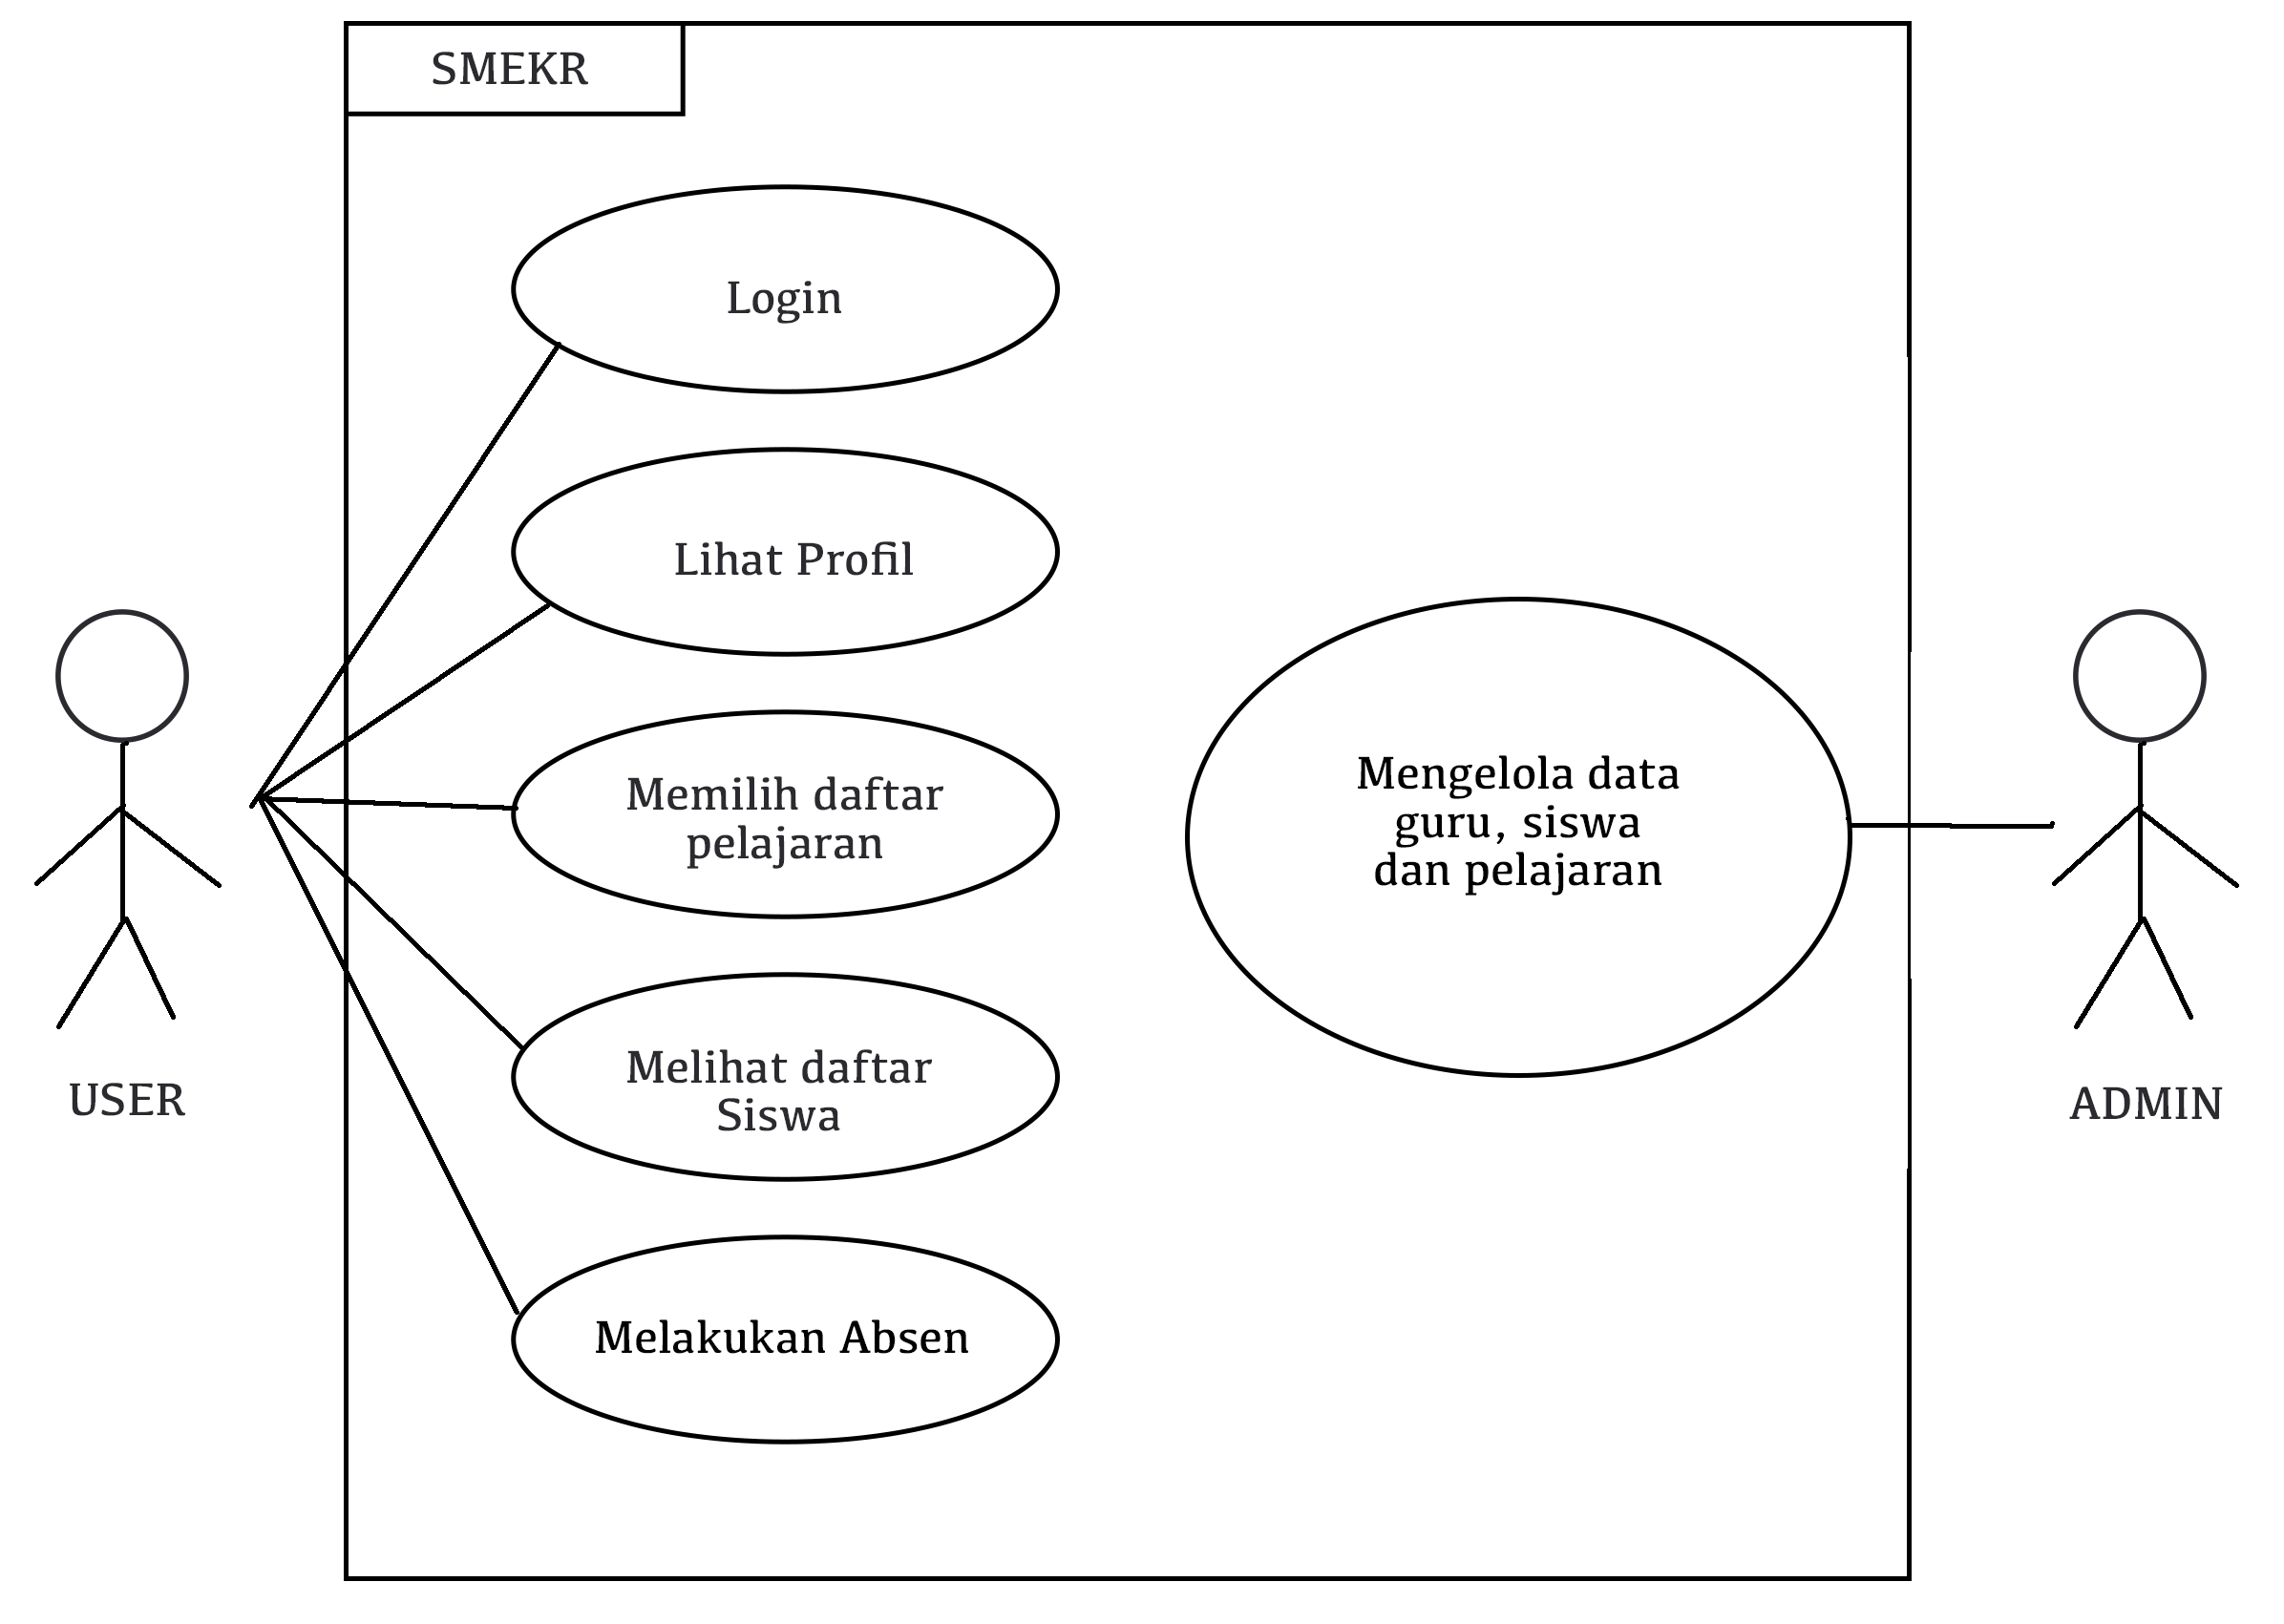
\includegraphics[width=9cm]{ussd}
\caption{Gambar Use Case Diagram}
\label{lab:use}
\end{figure}


\subsection{Diagram Activity}
Pada alur selanjutnya menjelaskan aktifitas alur \emph{user} dan sistem. Gambar \ref{lab:login}. menunjukan diagram \emph{activity} aplikasi.

\begin{figure}[h]
\centering
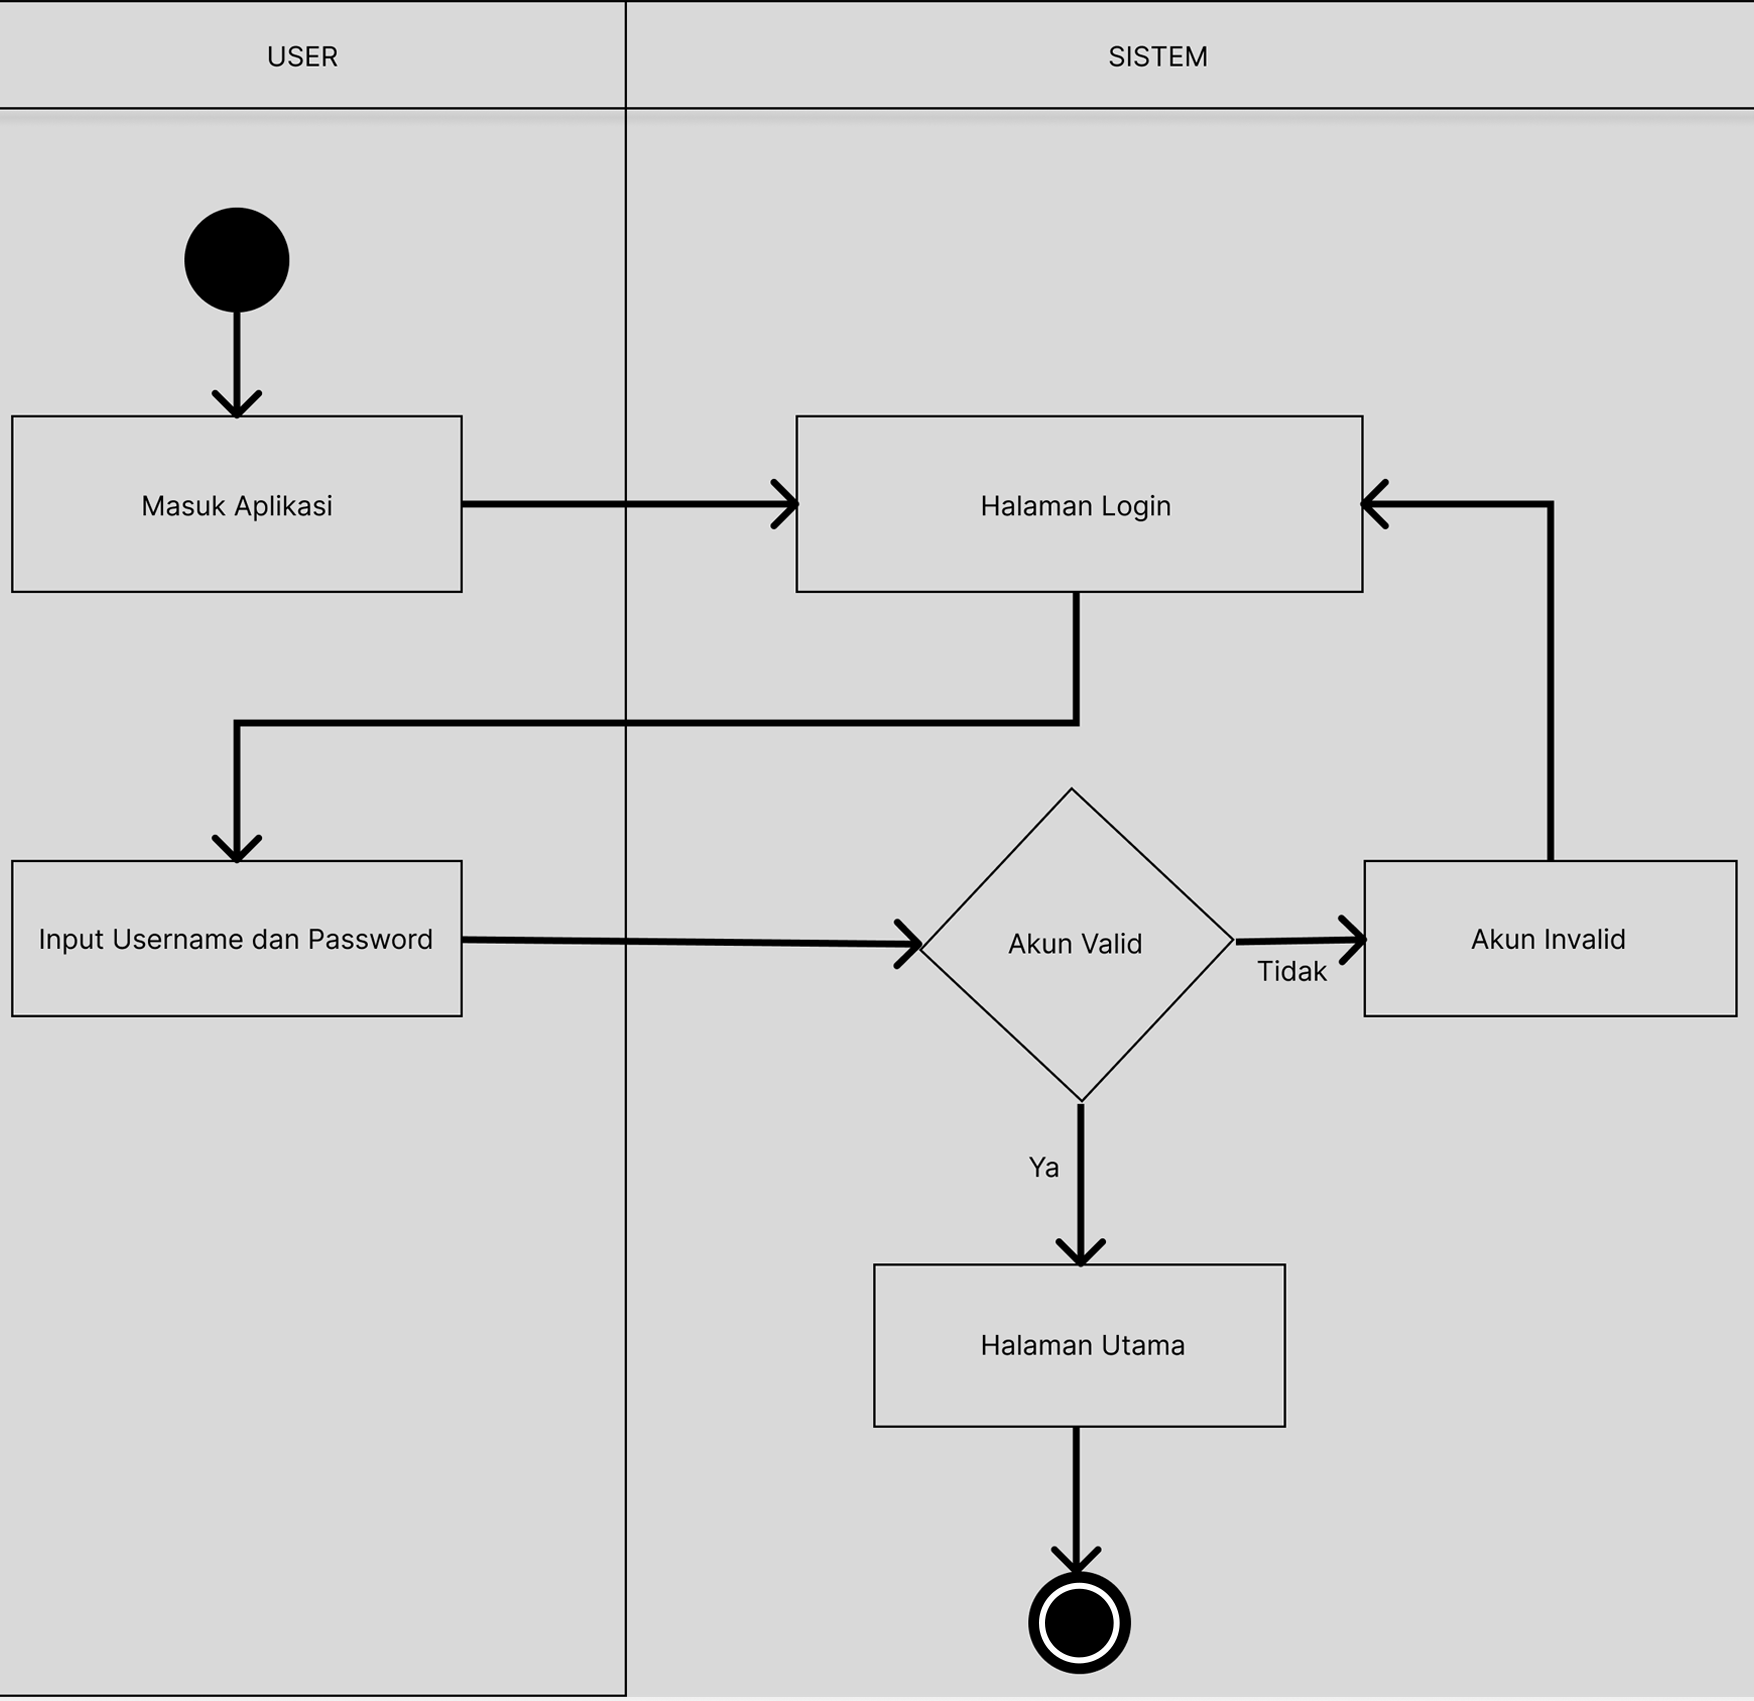
\includegraphics[width=14cm]{LOGIIN}
\caption{Gambar Diagram Activity Login}
\label{lab:login}
\end{figure}\
Pada gambar diatas menjelaskan proses \emph{login user} saat masuk ke dalam aplikasi, selanjutnya sistem menampilkan halaman \emph{login} dan \emph{user} memasukan \emph{username} dan \emph{password} yang sudah ditentukan oleh admin.
\newpage

\begin{figure}[h]
\centering
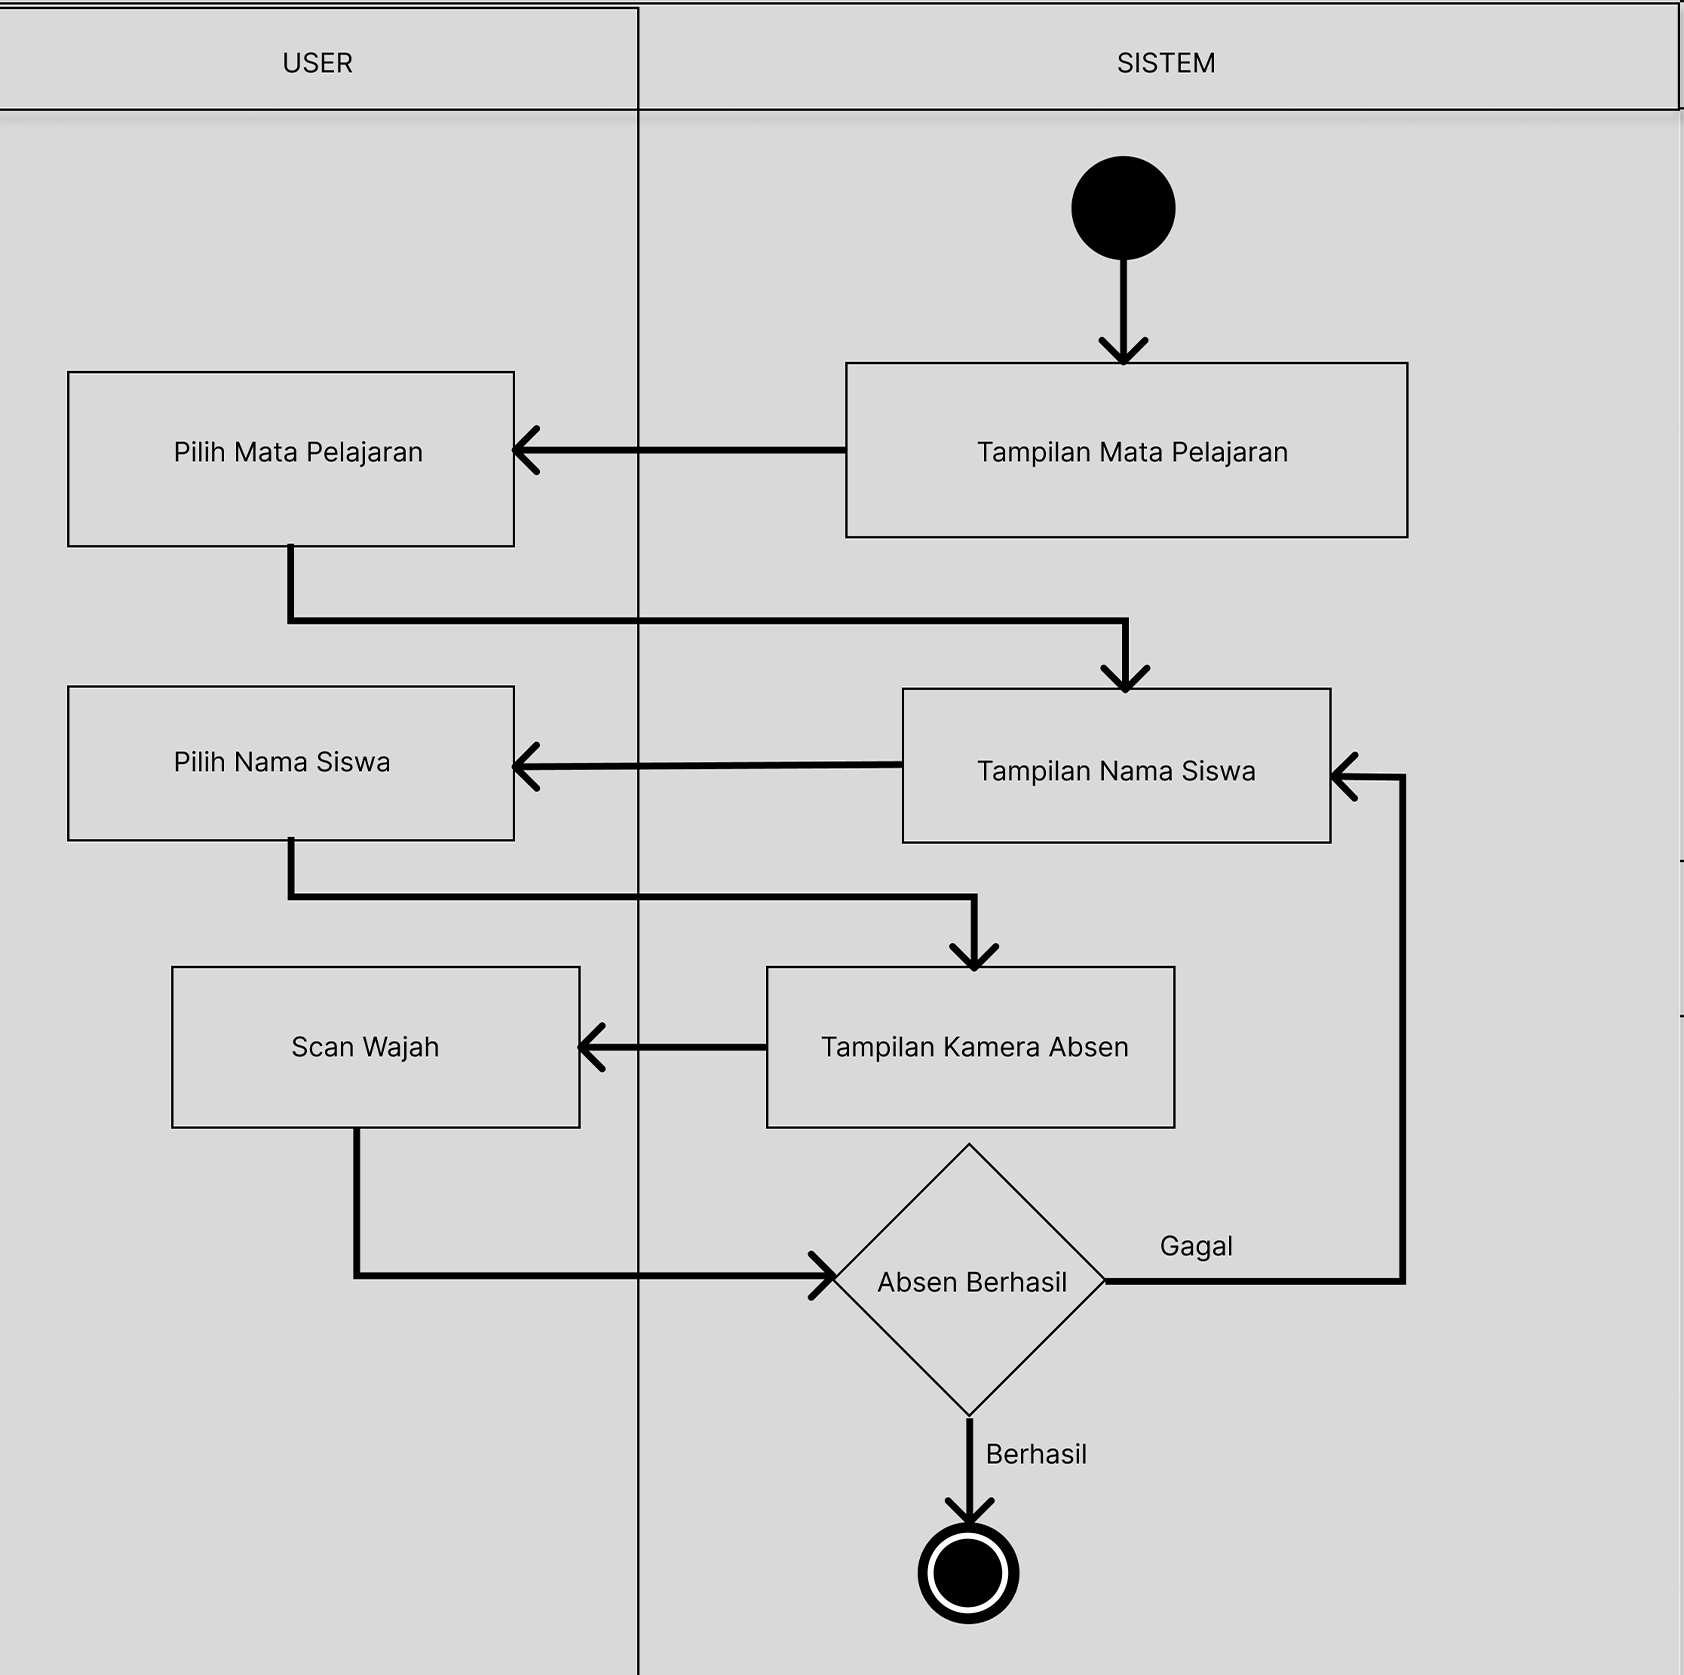
\includegraphics[width=14cm]{absen}
\caption{Gambar Diagram Activity Absen}
\label{lab:absen}
\end{figure}\
Pada gambar \ref{lab:absen} diatas menjelaskan proses presensi yang dilakukan \emph{user}, kemudian sistem menampilkan daftar siswa, \emph{user} melakukan \emph{scanning} wajah pada aplikasi, jika wajah sudah terdata maka presensi berhasil, jika tidak berhasil akan diarahkan oleh sistem untuk melakukan pemilihan ulang daftar siswa.
\newpage

\begin{figure}[h]
\centering
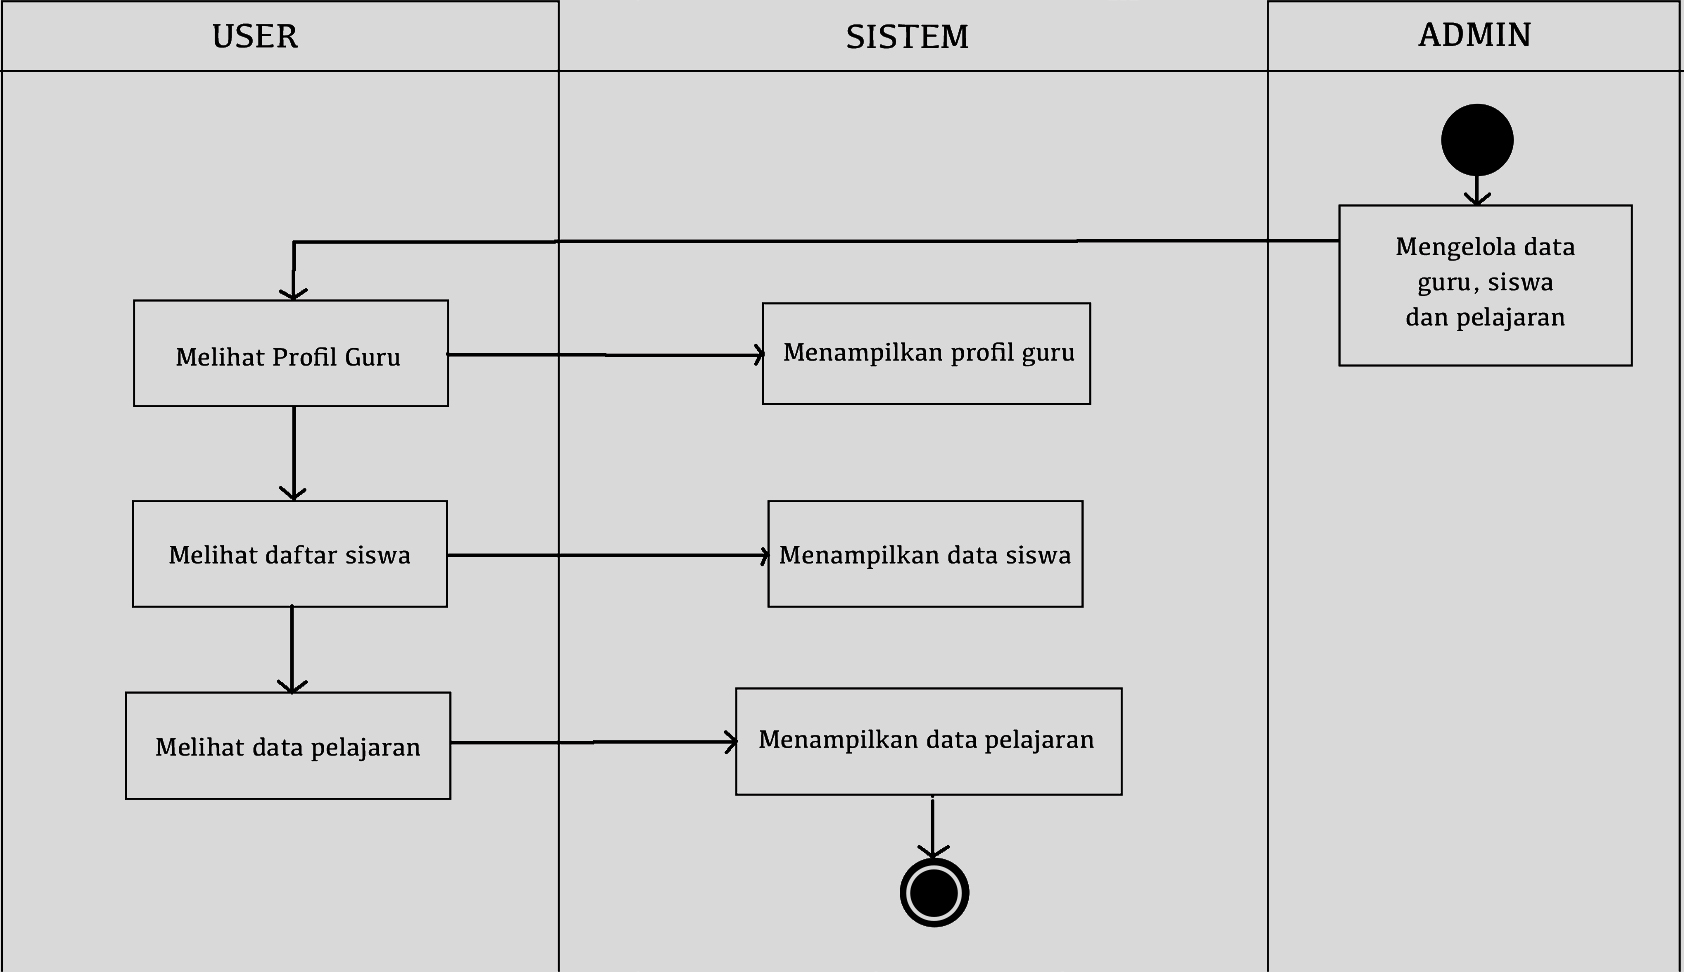
\includegraphics[width=14cm]{data}
\caption{Gambar Diagram Activity Data}
\label{lab:data}
\end{figure}\
Pada gambar \ref{lab:data}. diatas menjelaskan proses admin melakukan penambahan data, kemudian \emph{user} dapat melihat data yang telah diubah yang ditampilkan oleh sistem.
\newpage

\section{Metode Penelitian}
\subsection{Metodologi Penelitian}
Metodologi penelitian dapat dilihat pada gambar dibawah ini.
\begin{figure}[h]
\centering
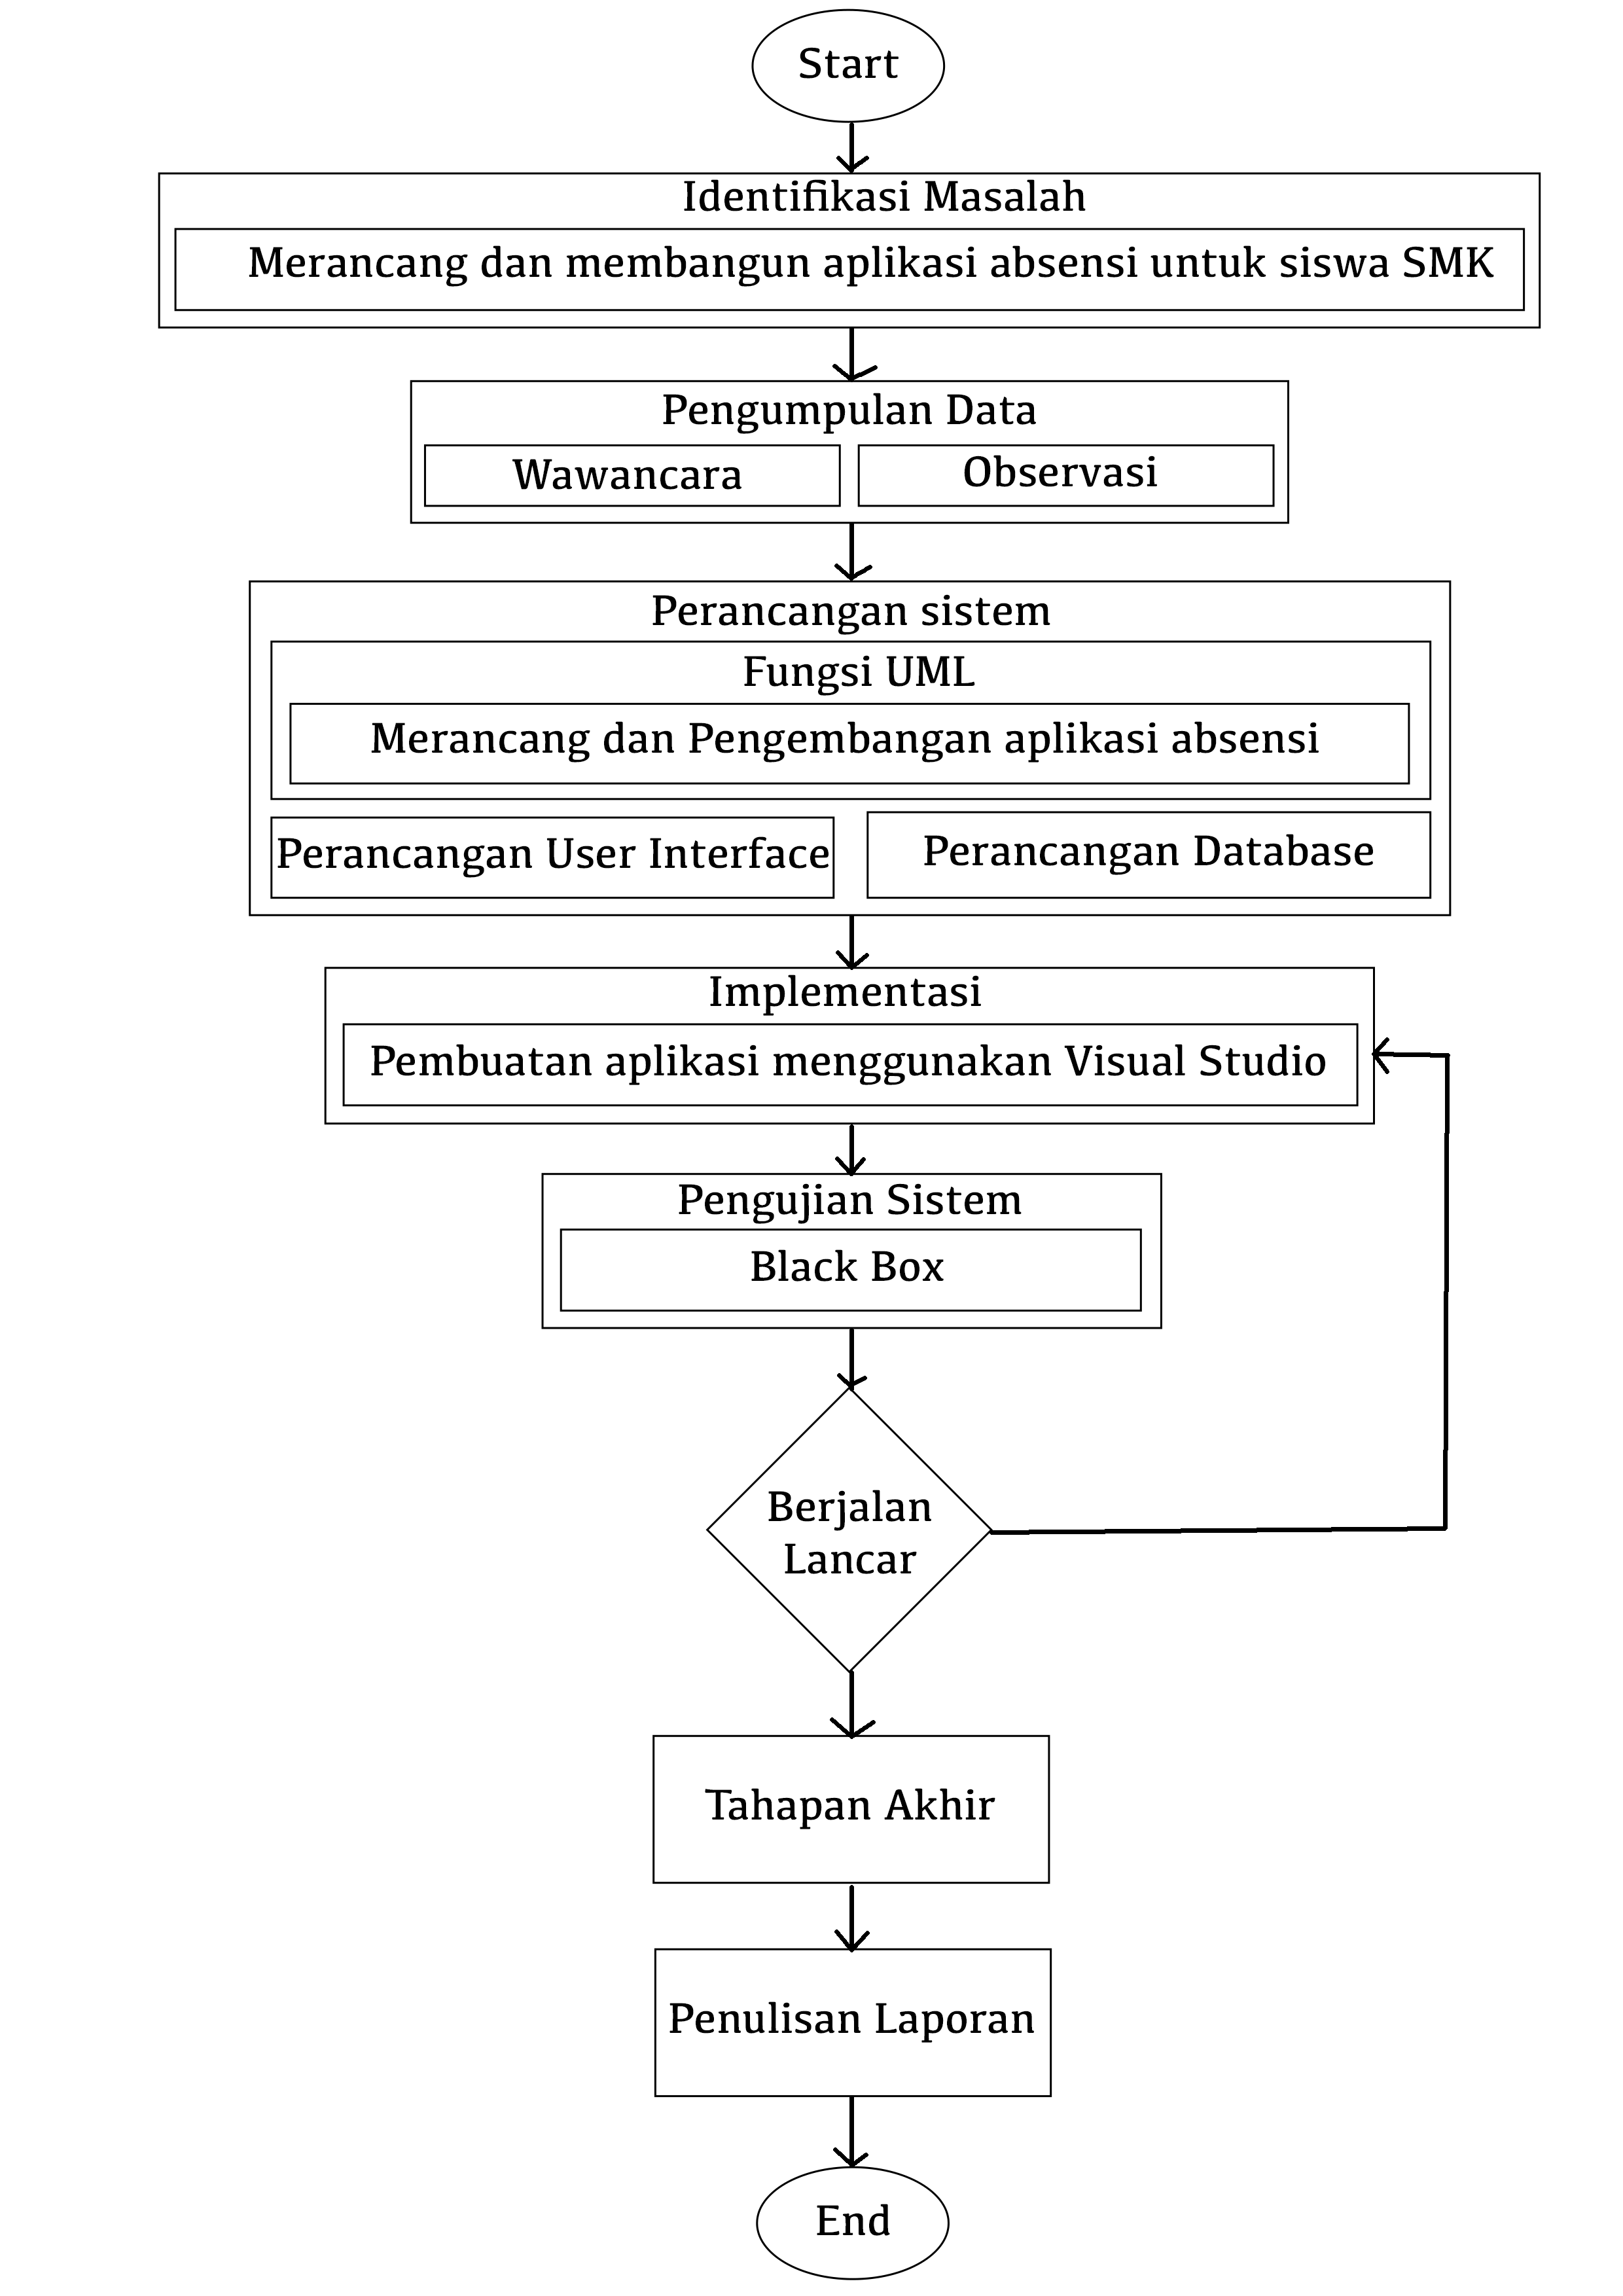
\includegraphics[width=11cm]{met}
\caption{Gambar Metodologi Penelitian}
\label{lab:met}
\end{figure}\
\newpage

\subsection{Perancangan Sistem}
Sistem yang digunakan berupa membaca struktur wajah saat melakukan absen, sistem presensi hanya berlaku didalam kelas menggunakan Smartphone guru.
\begin{enumerate}
\item Fungsional UML\\
Penulis merancang UML diagram, yaitu \emph{Use Case Diagram}
\item Perancangan \emph{User-Interface}\\
Menu yang ada didalam apliaksi meliputi, Login, presensi, data siswa, dan data mata pelajaran.
\item Perancangan \emph{Database}\\
Perancangan database berfungsi untuk menyimpan data siswa.
\end{enumerate} 

\subsection{Implementasi}
Perancangan yang sudah dibuat  di implementasikan menggunakan aplikasi visual studio hingga menjadi aplikasi presensi.

\section{Teknik Pengujian}
Tahapan pengujian dilakukan menggunakan \emph{black box} untuk menguji kelayakan aplikasi dan melihat terjadinya error menggunakan teknik \emph{Equivalence Partitioning} yaitu teknik yang bekerja dengan cara membagi data input dari beberapa perangkat lunak menjadi beberapa partisi data yang dibagi menjadi beberapa domain ke pengguna. Berikut contoh tabel pengujian \emph{black box}.


\section{Hasil yang diharapkan}
Dengan demikian, hasil yang diharapkan yaitu terciptanya aplikasi presensi dengan \emph{Face Recognition} yang akan mempermudah sistem presensi di SMK NEGERI 1 KARANG BARU.

\chapter*{JADWAL KEGIATAN PENELITIAN}
\addcontentsline{toc}{chapter}{JADWAL KEGIATAN PENELITIAN}


\begin{table}[!ht]
\caption{Jadwal Kegiatan}
\label{tab:jadwal-kegiatan}
\begin{tabular}{|c|m{5cm}|p{.2cm}|p{.2cm}|p{.2cm}|p{.2cm}|p{.2cm}|p{.2cm}|p{.2cm}|p{.2cm}|p{.2cm}|p{.2cm}|p{.2cm}|p{.2cm}|}
\hline
\multirow{2}{*}{No}	& 
\multicolumn{1}{c|}{\multirow{2}{*}{Kegiatan}}	& 
\multicolumn{4}{c|}{Mar} & 
\multicolumn{4}{c|}{Apr} &
\multicolumn{4}{c|}{Mei} \\ \cline{3-14}
& & 
\multicolumn{1}{c|}{1} &
\multicolumn{1}{c|}{2} &
\multicolumn{1}{c|}{3} &
\multicolumn{1}{c|}{4} &
\multicolumn{1}{c|}{1} &
\multicolumn{1}{c|}{2} &
\multicolumn{1}{c|}{3} &
\multicolumn{1}{c|}{4} &
\multicolumn{1}{c|}{1} &
\multicolumn{1}{c|}{2} &
\multicolumn{1}{c|}{3} &
\multicolumn{1}{c|}{4} \\ \hline
1  & Pengumpulan Data 			& \cellcolor{gray!75} & \cellcolor{gray!75} & & & & & & & & & & \\ \hline
2  & Identifikasi Masalah 		& & & \cellcolor{gray!75} & & & & & & & & & \\ \hline
3  & Analisis Kebutuhan Sistem 	& & \cellcolor{gray!75} & \cellcolor{gray!75} & \cellcolor{gray!75} & & & & & & & & \\ \hline
4  & Membuat Rancangan Sistem 	& & & & \cellcolor{gray!75} & \cellcolor{gray!75} & & & & & & & \\ \hline
5  & Rancang Bangun Program 	& & & & & & \cellcolor{gray!75} & \cellcolor{gray!75} & \cellcolor{gray!75} & & & & \\ \hline
6  & Uji coba program (\textit{testing}) 			& & & & & & & & \cellcolor{gray!75} & \cellcolor{gray!75} & & & \\ \hline
7  & Revisi Konsep, Desain Rancangan, Code Program & & & & & & & & & \cellcolor{gray!75} & \cellcolor{gray!75} & & \\ \hline
8  & Implementasi Program 					& & & & & & & & & & & \cellcolor{gray!75} & \\ \hline
9  & Pembimbingan Penulisan Naskah Skripsi & & & & & \cellcolor{gray!75} & \cellcolor{gray!75} & \cellcolor{gray!75} & \cellcolor{gray!75} & \cellcolor{gray!75} & & & \\ \hline
10 & Penulisan Akhir Laporan 				& & & & & & & & & & \cellcolor{gray!75} & & \\ \hline
11 & Pendadaran 							& & & & & & & & & & & & \cellcolor{gray!75} \\ \hline
\end{tabular}
\end{table}

\chapter*{RENCANA ANGGARAN PENELITIAN}
\addcontentsline{toc}{chapter}{RENCANA ANGGARAN PENELITIAN}


\begin{table}[!h]
\caption{Tabel Rencana Anggaran}
\centering
\begin{tabular}{|cccc|c|}
\hline
\multicolumn{1}{|c|}{\textbf{NO}} & \multicolumn{1}{c|}{\textbf{Material}} & \multicolumn{1}{c|}{\textbf{Jumlah}} & \textbf{Harga} & \textbf{Total} \\ \hline
\multicolumn{1}{|c|}{1}           & \multicolumn{1}{c|}{VPS}    & \multicolumn{1}{c|}{3 Bulan}         & Rp. 200.000    & Rp. 600.000    \\ \hline
\multicolumn{1}{|c|}{2}           & \multicolumn{1}{c|}{Pendataan}         & \multicolumn{1}{c|}{3 Bulan}         & Rp. 100.000    & Rp. 300.000    \\ \hline
\multicolumn{4}{|c|}{\textbf{Total}}                                                                                               & {\textbf{Rp. 900.000}}    \\ \hline
\end{tabular}
\end{table}

\begin{thebibliography}{9}
%\bibitem{tri}
%Tri Mulyono, Kusworo Adi dan Rahmat Gernowo 2012. \emph{SISTEM PENGENALAN WAJAH DENGAN METODE EIGENFACE DAN JARINGAN SYARAF TIRUAN (JST)}, Berkala Fisika ISSN : 1410 - 9662. Vol. 15, No. 1, Januari 2012, hal 15 - 20

\bibitem{nix}
Nixon Erzed, Nizirwan Anwar, Agung Mulyo Widodo, Eko Prasetyo, Kundang Karsono Juman 2022 \emph{Implementasi Flutter Pada Aplikasi Presensi Karyawan Berbasis Mobile}, P-ISSN :2580-4316, E-ISSN :2654-8054 https://journals.upi-yai.ac.id/index.php/ikraith-informatika/issue/archive

\bibitem{and}
Andi Maulidinnawati Abdul Kadir Parewe, A. Sumardin, Muhammad Isra Pratama \emph{Penerapan Metode Scrum dengan Framework Flutter dalam Teknologi Location based service Pada Sistem Provos Polisi}, Prosiding Seminar Nasional Teknik Elektro dan Informatika (SNTEI) 2022 – Teknik Informatika

\bibitem{k}
K. Hermawan, 2018. \emph{SIMULASI ENERGI OUTPUT MENGGUNAKAN APLIKASI CSharp DI PLTH BAYU BIRU YOGYAKARTA} 

\bibitem{ara}
Arafat Febriandirza, 2020. \emph{ERANCANGAN APLIKASI ABSENSI ONLINE DENGAN MENGGUNAKAN BAHASA PEMROGRAMAN KOTLIN}, Jurnal Pseudocode, Volume VII Nomor 2, September 2020, ISSN 2355-5920, e-ISSN 2655-1845 www.ejournal.unib.ac.id/index.php/pseudocode

\bibitem{l}
L. Septi and S. Wellia Shinta, 2015. \emph{Perancangan Aplikasi Mobile E-Commerce Berbasis Android Pada Violet Fashion Jepara}Sist. Inf., no. 5, p. 2.

\bibitem{dims}
Apa itu Android Studio dan Android SDK?, [Online]. Avaliable: https://www.dicoding.com/blog/apa-itu-android-studio-dan-android-sdk/ [Accesed 13 Maret 2023]

\bibitem{faz}
Fazriani Huzaimah, Dedy Irfan, 2018. \emph{RANCANG BANGUN APLIKASI UJIAN ONLINE PRA KOMPRE BERBASIS ANDROID}, VOTEKNIKA, Jurnal Vokasional Teknik Elektronika dan Informatika, http://ejournal.unp.ac.id/index.php/voteknika/index, Vol. 6, No. 2, Supplement (Juli – Desember 2018) E - ISSN: 2302-295

\bibitem{sten}
Stenly Ibrahim Adam, Oktoverano Lengkong, Stenly Pungus, 2021. \emph{Pengembangan Aplikasi Mobile Presensi Mahasiswa Berbasis QR-Code Di Universitas Klabat}. Cogito Smart Journal | VOL. 7 - NO.2, DESEMBER 2021.

\bibitem{gab}
Gabriella Genevine, Usman Rizal, 2015. \emph{ANALISIS PERBANDINGAN METODE TRANSFORMASI WAVELET DAN METODE EIGENFACE PADA PENGENALAN CITRA WAJAH DENGAN ANALISIS SWOT}, ISSN 2088-5555, Jurnal Manajemen Sistem Informasi Dan Teknologi Volume 05, Nomor 01, Juni 2015

\bibitem{susi}
Susi Tamba, 2022. \emph{Perancangan Aplikasi Absensi Karyawan Dengan Deteksi Wajah Menggunakan Metode Eigenface}, Journal of Informatics, Electrical and Electronics Engineering. ISSN 2807-9507 (Media Online), Vol 2, No 1, September 2022. Hal 12 - 17

\bibitem{jem}
JemyAgungPribadi, NinaSetiyawati, 2021. \emph{AbsenLoc: Aplikasi Absensi Mobile Berbasis Lokasi},  Jurnal Sistem dan Teknologi Informasi, p-ISSN : 2460-3562 / e-ISSN : 2620-8989, DOI: 10.26418/justin.v9i1.41103 Vol. 09, No. 1, Januari 2021

\end{thebibliography}
\addcontentsline{toc}{chapter}{DAFTAR PUSTAKA}

\end{document}
